% PrismSpace: System Flow, Architecture, DB Schema & Algorithm Presentation
\documentclass[aspectratio=169,10pt]{beamer}
\usetheme{Madrid}
\usecolortheme{default}
\usefonttheme{professionalfonts}
\usepackage[T1]{fontenc}
\usepackage{lmodern}
\usepackage{amsmath,amssymb}
\usepackage{booktabs}
\usepackage{tikz}
\usepackage{adjustbox}
\usepackage{tcolorbox}
\tcbuselibrary{skins}
\usepackage{fontawesome5}
\usepackage{tabularx}
\usepackage{array}
\usepackage{colortbl}
\usetikzlibrary{arrows.meta,positioning,fit,backgrounds,calc,shadows,shapes.geometric}

\providecommand{\pk}[1]{\textbf{#1}}
\providecommand{\idx}[1]{\textit{#1}}
\providecommand{\comp}[1]{\texttt{#1}}

% Lavender Color Palette for Professional Headers & Visual Flow
\definecolor{lavenderDark}{RGB}{76, 51, 122}      % #4C337A - Deep Royal Lavender for Frametitles, Banners, Headers
\definecolor{lavenderDeep}{RGB}{58, 36, 96}       % #3A2460 - High-contrast lavender for text on light backgrounds
\definecolor{lavenderMedium}{RGB}{124, 98, 173}   % #7C62AD - Medium Lavender for Subheaders, Footers, Accents
\definecolor{lavenderLight}{RGB}{243, 239, 252}   % #F3EFFC - Soft Lavender Mist for fills and backgrounds
\definecolor{lavenderBorder}{RGB}{186, 168, 224}  % #BAA8E0 - Soft Lavender border
\definecolor{lavenderAccent}{RGB}{150, 120, 205}  % #9678CD - Accent lilac for highlights & bullets

% PrismSpace Supporting Palette
\definecolor{bannerGreen}{RGB}{76, 51, 122}      % mapped to lavenderDark
\definecolor{prismNavy}{RGB}{76, 51, 122}        % mapped to lavenderDark for headers
\definecolor{prismBlue}{RGB}{124, 98, 173}       % mapped to lavenderMedium
\definecolor{prismTeal}{RGB}{22,138,114}
\definecolor{prismMint}{RGB}{243, 239, 252}
\definecolor{prismGold}{RGB}{217,154,34}
\definecolor{prismDark}{RGB}{23,32,42}
\definecolor{prismLight}{RGB}{248,247,252}       % subtle soft lavender-tinted light bg
\definecolor{prismIndigo}{RGB}{76, 51, 122}
\definecolor{prismSlate}{RGB}{102,112,133}
\definecolor{cardBg}{RGB}{255,255,255}

% Harmonious pastel node fills for Architecture Diagram
\definecolor{cInput}{RGB}{231,233,236}
\definecolor{cStem}{RGB}{220,214,247}
\definecolor{cStage1}{RGB}{191,232,213}
\definecolor{cStage2}{RGB}{246,213,138}
\definecolor{cStage3}{RGB}{242,184,181}
\definecolor{cStage4}{RGB}{191,227,242}
\definecolor{cHead}{RGB}{216,197,232}
\definecolor{cOutput}{RGB}{234,207,213}
% Detailed execution-core fills from page 03 palette
\definecolor{cTask}{RGB}{231,233,236}
\definecolor{cPlanner}{RGB}{207,199,242}
\definecolor{cDispatch}{RGB}{169,220,235}
\definecolor{cReact}{RGB}{169,222,200}
\definecolor{cTool}{RGB}{244,213,141}
\definecolor{cSafety}{RGB}{240,170,167}
\definecolor{cMemory}{RGB}{214,185,230}
\definecolor{cDeliverable}{RGB}{185,222,210}

% Beamer Palette Settings - Lavender Theme
\setbeamercolor{structure}{fg=lavenderDark}
\setbeamercolor{background canvas}{bg=prismLight}
\setbeamercolor{normal text}{fg=prismDark,bg=prismLight}
\setbeamercolor{frametitle}{bg=lavenderDark,fg=white}
\setbeamercolor{title}{fg=lavenderDark}
\setbeamercolor{author}{fg=lavenderMedium}
\setbeamercolor{institute}{fg=gray}
\setbeamercolor{date}{fg=gray}

\setbeamercolor{block title}{bg=lavenderDark,fg=white}
\setbeamercolor{block body}{bg=cardBg,fg=prismDark}

\setbeamercolor{block title alerted}{bg=prismGold!90!black,fg=white}
\setbeamercolor{block body alerted}{bg=prismGold!10,fg=prismDark}

\setbeamercolor{block title example}{bg=lavenderMedium,fg=white}
\setbeamercolor{block body example}{bg=lavenderLight,fg=prismDark}

\setbeamertemplate{navigation symbols}{}

% Professional Header and Footer with Lavender Palette
\setbeamercolor{author in head/foot}{bg=lavenderDark, fg=white}
\setbeamercolor{title in head/foot}{bg=lavenderMedium, fg=white}
\setbeamercolor{date in head/foot}{bg=lavenderDark, fg=white}
\setbeamertemplate{footline}
{
  \leavevmode%
  \hbox{%
  \begin{beamercolorbox}[wd=.28\paperwidth,ht=2.5ex,dp=1.1ex,center]{author in head/foot}%
    \usebeamerfont{author in head/foot}\textbf{Group 01} $\cdot$ CSE, CEK
  \end{beamercolorbox}%
  \begin{beamercolorbox}[wd=.48\paperwidth,ht=2.5ex,dp=1.1ex,center]{title in head/foot}%
    \usebeamerfont{title in head/foot}\textbf{PrismSpace}: Architecture, Flow, DB \& Algorithm
  \end{beamercolorbox}%
  \begin{beamercolorbox}[wd=.24\paperwidth,ht=2.5ex,dp=1.1ex,right]{date in head/foot}%
    \usebeamerfont{date in head/foot}\insertframenumber{} / \inserttotalframenumber\hspace*{2ex} 
  \end{beamercolorbox}}%
  \vskip0pt%
}

\setbeamertemplate{itemize item}{\color{lavenderAccent}$\blacktriangleright$}
\setbeamertemplate{itemize subitem}{\color{lavenderMedium}$\bullet$}
\setbeamertemplate{itemize subsubitem}{\color{prismGold}$-$}

% Title Metadata
\title[PrismSpace]{\textbf{\LARGE PrismSpace}}
\subtitle{\large System Flow, Multi-Layer Architecture, Browser DB Schema \& Swarm Algorithms}
\author[Group 01]{
  \textbf{Nobin Sijo} \and \textbf{Pranav P} \and \textbf{Prasanth P} \and \textbf{Sankar Narayan S}
}
\institute[CEK]{
  \textbf{Department of Computer Science \& Engineering}\\
  College of Engineering, Karunagappally
}
\date{\today}

\begin{document}

% =============================================================================
% TITLE SLIDE (Matches Reference Layout)
% =============================================================================
\begin{frame}[plain]
\begin{tikzpicture}[remember picture,overlay]
  % 1. Top Lavender Banner with Drop Shadow
  \node[
    rounded corners=5pt,
    fill=lavenderDark,
    drop shadow={shadow xshift=1.5pt, shadow yshift=-2.0pt, opacity=0.35},
    minimum width=15.2cm,
    minimum height=0.98cm,
    inner sep=0pt
  ] at ([yshift=-0.78cm]current page.north) {};

  \node[text=white, font=\bfseries\fontsize{13.5}{16}\selectfont] at ([yshift=-0.78cm]current page.north) {
    PRISMSPACE - INTELLIGENT MULTI-AGENT PLATFORM
  };

  % 2. College Emblem
  \node at ([yshift=-1.95cm]current page.north) {
    
\includegraphics[height=0.95cm]{cek-logo.png}
  };

  % 3. Department & College Text
  \node[font=\footnotesize, align=center] at ([yshift=-2.82cm]current page.north) {
    \textbf{Dept. of Computer Science \& Engineering}\\[0.12em]
    College of Engineering, Karunagappally
  };

  % 4. Project Group Header
  \node[font=\large\bfseries, text=lavenderDark] at ([yshift=-3.55cm]current page.north) {
    Project Group 01
  };

  % 5. Students & Register Numbers Table
  \node[font=\small] at ([yshift=-4.60cm]current page.north) {
    \begin{tabular}{l@{\hspace{3.4cm}}l}
      \textbf{NOBIN SIJO}        & KNP23CS082 \\
      \textbf{PRANAV P}          & KNP23CS085 \\
      \textbf{PRASANTH P}        & KNP23CS086 \\
      \textbf{SANKAR NARAYAN S}  & KNP23CS094
    \end{tabular}
  };

  % 6. Horizontal Lavender Accent Line
  \draw[lavenderDark, line width=0.9pt] ([xshift=1.6cm, yshift=-5.58cm]current page.north west) -- ([xshift=-1.6cm, yshift=-5.58cm]current page.north east);

  % 7. Project Coordinator & Guide Details (Centered)
  \node[align=center, font=\footnotesize] at ([yshift=-6.70cm]current page.north) {
    {\color{lavenderDark}\textit{Project Coordinator \& Guide}}\\[0.25em]
    \textbf{\small Dr. Leena Silvoster}\\[0.12em]
    Associate Professor\\[0.08em]
    College of Engineering, Karunagappally
  };
\end{tikzpicture}
\end{frame}

% =============================================================================
% SECTION 1: SYSTEM FLOW
% =============================================================================
\section{System Flow}

\begin{frame}[t]{01. Overall End-to-End System Flow (Figure 4.3)}
\vspace{0.12cm}
\centering
\adjustbox{max height=0.86\textheight, max width=0.98\linewidth}{%
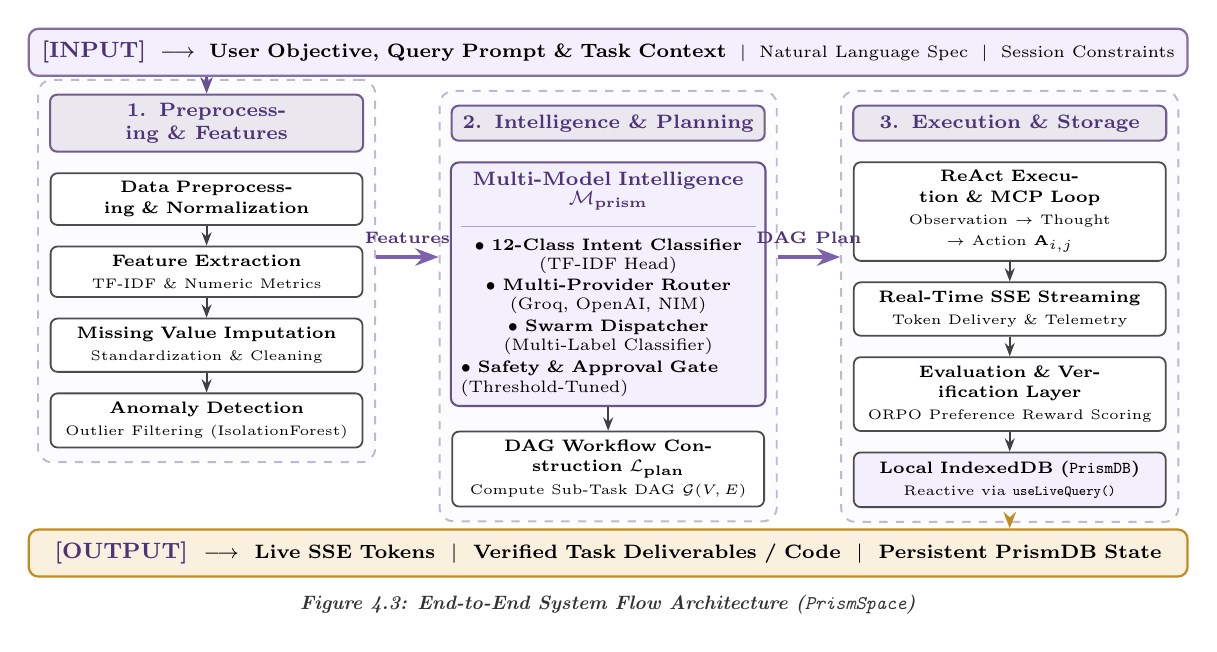
\begin{tikzpicture}[
    x=1cm, y=1cm,
    font=\sffamily,
    inout/.style={
        rectangle, rounded corners=3.5pt, line width=0.8pt,
        inner sep=4.5pt, align=center,
        font=\fontsize{7.2}{8.8}\selectfont
    },
    hdrbox/.style={
        rectangle, draw=lavenderDark!80, line width=0.75pt, fill=lavenderDark!12,
        rounded corners=2.5pt, inner sep=3.2pt, align=center,
        text width=3.75cm,
        font=\fontsize{6.8}{8.0}\selectfont\bfseries\color{lavenderDark}
    },
    stepbox/.style={
        rectangle, draw=black!70, line width=0.65pt, fill=white,
        rounded corners=2.5pt, inner sep=3.0pt, align=center,
        text width=3.75cm,
        font=\fontsize{6.2}{7.4}\selectfont
    },
    enginebox/.style={
        rectangle, draw=lavenderDark!85, line width=0.75pt, fill=lavenderLight,
        rounded corners=3pt, inner sep=3.5pt, align=left,
        text width=3.75cm,
        font=\fontsize{5.8}{7.0}\selectfont
    },
    stagebox/.style={
        rectangle, draw=lavenderDark!35, dashed, rounded corners=5pt, line width=0.7pt,
        fill=lavenderLight!25, inner xsep=4pt, inner ysep=5pt
    },
    flowarr/.style={
        -{Stealth[scale=0.75]}, line width=0.75pt, draw=black!75
    },
    transarr/.style={
        -{Stealth[scale=0.95]}, line width=1.3pt, draw=lavenderMedium
    }
]

    % =========================================================================
    % 1. TOP: EXPLICIT INPUT BAR (Lavender Theme)
    % =========================================================================
    \node [inout, fill=lavenderLight, draw=lavenderDark!70, text width=14.4cm] (input_node) at (0, 3.0) {
        \textbf{\fontsize{7.8}{9.2}\selectfont\color{lavenderDark}[INPUT]} $\;\longrightarrow\;$
        \textbf{User Objective, Query Prompt \& Task Context}
        {\fontsize{6.5}{7.8}\selectfont $\;\vert\;$ Natural Language Spec $\;\vert\;$ Session Constraints}
    };

    % =========================================================================
    % 2. MIDDLE: 3-STAGE HORIZONTAL PIPELINE
    % =========================================================================

    % --- STAGE 1: INGESTION & DATA PREPROCESSING ---
    \node [hdrbox] (h1) at (-5.1, 2.1) {1. Preprocessing \& Features};
    \node [stepbox, below=0.25cm of h1] (s1_1) {\textbf{Data Preprocessing \& Normalization}};
    \node [stepbox, below=0.25cm of s1_1] (s1_2) {
        \textbf{Feature Extraction}\\[0.1em]
        {\fontsize{5.4}{6.4}\selectfont TF-IDF \& Numeric Metrics}
    };
    \node [stepbox, below=0.25cm of s1_2] (s1_3) {
        \textbf{Missing Value Imputation}\\[0.1em]
        {\fontsize{5.4}{6.4}\selectfont Standardization \& Cleaning}
    };
    \node [stepbox, below=0.25cm of s1_3] (s1_4) {
        \textbf{Anomaly Detection}\\[0.1em]
        {\fontsize{5.4}{6.4}\selectfont Outlier Filtering (IsolationForest)}
    };

    \draw [flowarr] (s1_1) -- (s1_2);
    \draw [flowarr] (s1_2) -- (s1_3);
    \draw [flowarr] (s1_3) -- (s1_4);

    \begin{scope}[on background layer]
    \node [stagebox, fit=(h1) (s1_4)] (stage1) {};
    \end{scope}

    % --- STAGE 2: MULTI-MODEL INTELLIGENCE & DAG PLANNING ---
    \node [hdrbox] (h2) at (0, 2.1) {2. Intelligence \& Planning};
    \node [enginebox, below=0.25cm of h2] (s2_1) {
        \centering\textbf{\fontsize{6.8}{8.0}\selectfont\color{lavenderDark}Multi-Model Intelligence $\mathcal{M}_{\text{prism}}$}\\[0.15em]
        {\color{lavenderMedium!60}\rule{\linewidth}{0.4pt}}\\[0.2em]
        {\fontsize{5.6}{6.8}\selectfont
        $\bullet$ \textbf{12-Class Intent Classifier} (TF-IDF Head)\\[0.15em]
        $\bullet$ \textbf{Multi-Provider Router} (Groq, OpenAI, NIM)\\[0.15em]
        $\bullet$ \textbf{Swarm Dispatcher} (Multi-Label Classifier)\\[0.15em]
        $\bullet$ \textbf{Safety \& Approval Gate} (Threshold-Tuned)}
    };

    \node [stepbox, below=0.30cm of s2_1] (s2_2) {
        \textbf{DAG Workflow Construction $\mathcal{L}_{\text{plan}}$}\\[0.12em]
        {\fontsize{5.4}{6.4}\selectfont Compute Sub-Task DAG $\mathcal{G}(V, E)$}
    };

    \draw [flowarr] (s2_1) -- (s2_2);

    \begin{scope}[on background layer]
    \node [stagebox, fit=(h2) (s2_2)] (stage2) {};
    \end{scope}

    % --- STAGE 3: EXECUTION, STREAMING & PERSISTENCE ---
    \node [hdrbox] (h3) at (5.1, 2.1) {3. Execution \& Storage};
    \node [stepbox, below=0.25cm of h3] (s3_1) {
        \textbf{\fontsize{6.2}{7.3}\selectfont ReAct Execution \& MCP Loop}\\[0.1em]
        {\fontsize{5.4}{6.4}\selectfont Observation $\to$ Thought $\to$ Action $\mathbf{A}_{i,j}$}
    };
    \node [stepbox, below=0.25cm of s3_1] (s3_2) {
        \textbf{Real-Time SSE Streaming}\\[0.1em]
        {\fontsize{5.4}{6.4}\selectfont Token Delivery \& Telemetry}
    };
    \node [stepbox, below=0.25cm of s3_2] (s3_3) {
        \textbf{Evaluation \& Verification Layer}\\[0.1em]
        {\fontsize{5.4}{6.4}\selectfont ORPO Preference Reward Scoring}
    };
    \node [stepbox, below=0.25cm of s3_3, fill=lavenderLight] (s3_4) {
        \textbf{Local IndexedDB (\texttt{PrismDB})}\\[0.1em]
        {\fontsize{5.4}{6.4}\selectfont Reactive via \texttt{useLiveQuery()}}
    };

    \draw [flowarr] (s3_1) -- (s3_2);
    \draw [flowarr] (s3_2) -- (s3_3);
    \draw [flowarr] (s3_3) -- (s3_4);

    \begin{scope}[on background layer]
    \node [stagebox, fit=(h3) (s3_4)] (stage3) {};
    \end{scope}

    % --- PIPELINE TRANSITIONS BETWEEN STAGES (Strictly horizontal with clearance) ---
    \draw [transarr] ($(stage1.east |- 0, 0.4)$) -- 
        node[above=1pt, font=\fontsize{6.0}{7.0}\selectfont\bfseries\color{lavenderDark}]{Features} ($(stage2.west |- 0, 0.4)$);

    \draw [transarr] ($(stage2.east |- 0, 0.4)$) -- 
        node[above=1pt, font=\fontsize{6.0}{7.0}\selectfont\bfseries\color{lavenderDark}]{DAG Plan} ($(stage3.west |- 0, 0.4)$);

    % Connect Input cleanly to Stage 1 Header
    \draw [flowarr, line width=1.1pt, draw=lavenderDark!85] (input_node.south -| h1.north) -- (h1.north);

    % =========================================================================
    % 3. BOTTOM: EXPLICIT OUTPUT BAR
    % =========================================================================
    \node [inout, fill=prismGold!15, draw=prismGold!90!black, text width=14.4cm, below=0.45cm of $(stage1.south)!0.5!(stage3.south)$] (output_node) {
        \textbf{\fontsize{7.8}{9.2}\selectfont\color{lavenderDark}[OUTPUT]} $\;\longrightarrow\;$
        \textbf{Live SSE Tokens} $\;\vert\;$
        \textbf{Verified Task Deliverables / Code} $\;\vert\;$
        \textbf{Persistent PrismDB State}
    };

    % Connect Stage 3 cleanly to Output
    \draw [flowarr, line width=1.1pt, draw=prismGold!90!black] (stage3.south -| h3.south) -- (output_node.north -| h3.south);

    % Caption
    \node [font=\fontsize{7.2}{8.5}\selectfont\bfseries\color{black!80}, below=0.10cm of output_node] {
        \textit{Figure 4.3: End-to-End System Flow Architecture (\texttt{PrismSpace})}
    };

\end{tikzpicture}%
}
\end{frame}


% =============================================================================
% SECTION 2: SYSTEM ARCHITECTURE & WORKFLOW
% =============================================================================
\section{System Architecture}

\begin{frame}[t]{02. System Architecture: 6-Tier Stack \& Multi-Agent Workflow}
\vspace{-0.4em}
\centering
\adjustbox{max width=0.99\linewidth, max height=0.76\textheight}{%
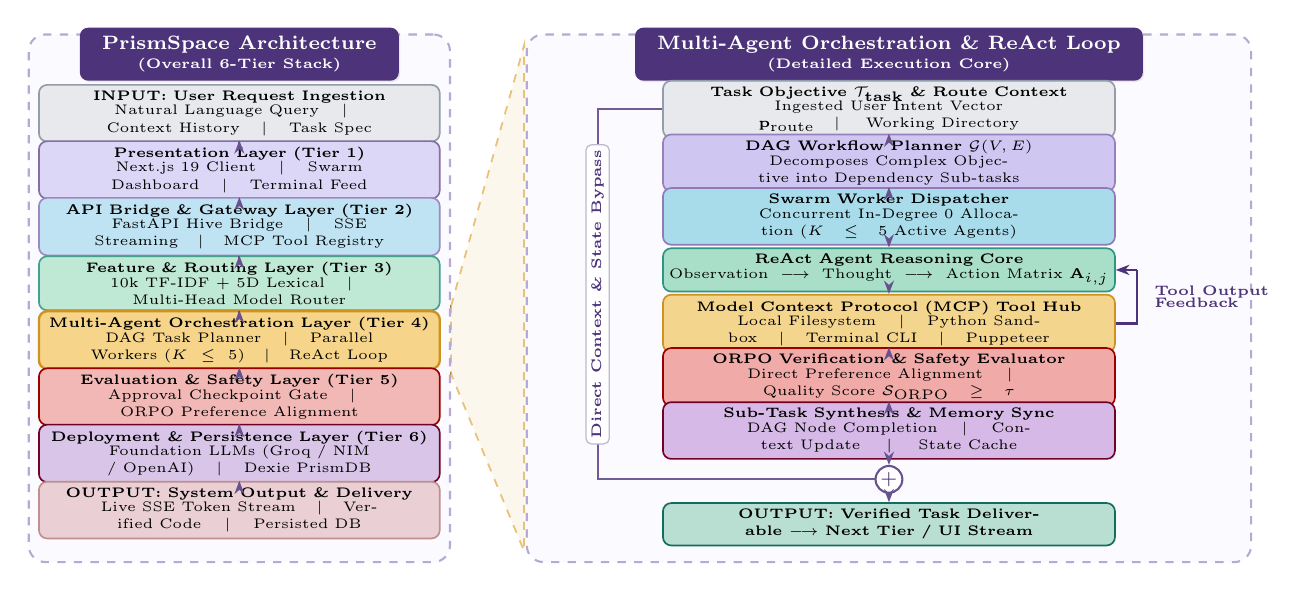
\begin{tikzpicture}[
  x=1cm, y=1cm,
  every node/.style={align=center},
  card/.style={
    draw=lavenderMedium!55, dashed, line width=0.75pt, fill=lavenderLight!30,
    rounded corners=6pt
  },
  pilltitle/.style={
    fill=lavenderDark, text=white, font=\scriptsize\bfseries,
    rounded corners=3pt, inner xsep=8pt, inner ysep=3.2pt,
    drop shadow={opacity=0.15, shadow xshift=0.5pt, shadow yshift=-0.5pt}
  },
  layerbox/.style={
    rectangle, rounded corners=3pt, line width=0.6pt,
    text width=4.95cm, minimum height=0.45cm, inner ysep=2.2pt, inner xsep=2pt,
    font=\fontsize{5.2}{6.2}\selectfont
  },
  detailbox/.style={
    rectangle, rounded corners=3pt, line width=0.6pt,
    text width=5.6cm, minimum height=0.45cm, inner ysep=2.2pt, inner xsep=2pt,
    font=\fontsize{5.2}{6.2}\selectfont
  },
  arrow/.style={
    -{Stealth[scale=0.75]}, line width=0.75pt, draw=lavenderDark!85
  },
  conn/.style={
    draw=lavenderDark!80, line width=0.75pt
  },
  plusnode/.style={
    circle, draw=lavenderDark!85, line width=0.75pt, fill=white,
    inner sep=0pt, minimum size=0.34cm, font=\scriptsize\bfseries, text=lavenderDark
  }
]

  % =========================================================================
  % LEFT CONTAINER: OVERALL 6-TIER ARCHITECTURE
  % Card 1: center=(2.85, 3.25), width=5.35cm, height=6.70cm => x in [0.175, 5.525]
  % =========================================================================
  \node[card, minimum width=5.35cm, minimum height=6.70cm] (card1) at (2.85, 3.25) {};
  \node[pilltitle] (title1) at (2.85, 6.35) {PrismSpace Architecture\\[-0.15em]{\fontsize{4.8}{5.8}\selectfont (Overall 6-Tier Stack)}};

  \node[layerbox, fill=cInput, draw=prismSlate!70] (l0) at (2.85, 5.60) {
    \textbf{INPUT: User Request Ingestion}\\[-0.15em]
    \fontsize{4.5}{5.5}\selectfont Natural Language Query $\;\vert\;$ Context History $\;\vert\;$ Task Spec
  };

  \node[layerbox, fill=cStem, draw=prismIndigo!70] (l1) at (2.85, 4.88) {
    \textbf{Presentation Layer (Tier 1)}\\[-0.15em]
    \fontsize{4.5}{5.5}\selectfont Next.js 19 Client $\;\vert\;$ Swarm Dashboard $\;\vert\;$ Terminal Feed
  };

  \node[layerbox, fill=cStage4, draw=prismBlue!75] (l2) at (2.85, 4.16) {
    \textbf{API Bridge \& Gateway Layer (Tier 2)}\\[-0.15em]
    \fontsize{4.5}{5.5}\selectfont FastAPI Hive Bridge $\;\vert\;$ SSE Streaming $\;\vert\;$ MCP Tool Registry
  };

  \node[layerbox, fill=cStage1, draw=prismTeal!80] (l3) at (2.85, 3.44) {
    \textbf{Feature \& Routing Layer (Tier 3)}\\[-0.15em]
    \fontsize{4.5}{5.5}\selectfont 10k TF-IDF + 5D Lexical $\;\vert\;$ Multi-Head Model Router
  };

  \node[layerbox, fill=cStage2, draw=prismGold!95!black, line width=0.85pt] (l4) at (2.85, 2.72) {
    \textbf{Multi-Agent Orchestration Layer (Tier 4)}\\[-0.15em]
    \fontsize{4.5}{5.5}\selectfont DAG Task Planner $\;\vert\;$ Parallel Workers ($K \le 5$) $\;\vert\;$ ReAct Loop
  };

  \node[layerbox, fill=cStage3, draw=red!60!black] (l5) at (2.85, 2.00) {
    \textbf{Evaluation \& Safety Layer (Tier 5)}\\[-0.15em]
    \fontsize{4.5}{5.5}\selectfont Approval Checkpoint Gate $\;\vert\;$ ORPO Preference Alignment
  };

  \node[layerbox, fill=cHead, draw=purple!60!black] (l6) at (2.85, 1.28) {
    \textbf{Deployment \& Persistence Layer (Tier 6)}\\[-0.15em]
    \fontsize{4.5}{5.5}\selectfont Foundation LLMs (Groq / NIM / OpenAI) $\;\vert\;$ Dexie PrismDB
  };

  \node[layerbox, fill=cOutput, draw=pink!75!black] (l7) at (2.85, 0.56) {
    \textbf{OUTPUT: System Output \& Delivery}\\[-0.15em]
    \fontsize{4.5}{5.5}\selectfont Live SSE Token Stream $\;\vert\;$ Verified Code $\;\vert\;$ Persisted DB
  };

  % Downward arrows on Left Card
  \draw[arrow] (l0) -- (l1);
  \draw[arrow] (l1) -- (l2);
  \draw[arrow] (l2) -- (l3);
  \draw[arrow] (l3) -- (l4);
  \draw[arrow] (l4) -- (l5);
  \draw[arrow] (l5) -- (l6);
  \draw[arrow] (l6) -- (l7);

  % =========================================================================
  % RIGHT CONTAINER: DETAILED VIEW (MULTI-AGENT ORCHESTRATION & REACT LOOP)
  % Card 2: center=(11.10, 3.25), width=9.20cm, height=6.70cm => x in [6.50, 15.70]
  % Gap between Card 1 & Card 2: [5.48, 6.50] = 1.02cm
  % Boxes centered at x=11.10, width=5.60cm => x in [8.30, 13.90]
  % Left corridor: [6.50, 8.30] = 1.80cm (Bypass line at x=7.40)
  % Right corridor: [13.90, 15.70] = 1.80cm (Feedback line at x=14.25)
  % =========================================================================
  \node[card, minimum width=9.20cm, minimum height=6.70cm] (card2) at (11.10, 3.25) {};
  \node[pilltitle] (title2) at (11.10, 6.35) {Multi-Agent Orchestration \& ReAct Loop\\[-0.15em]{\fontsize{4.8}{5.8}\selectfont (Detailed Execution Core)}};

  \node[detailbox, fill=cTask, draw=prismSlate!70] (d_in) at (11.10, 5.65) {
    \textbf{Task Objective $\mathcal{T}_{\text{task}}$ \& Route Context}\\[-0.15em]
    \fontsize{4.5}{5.5}\selectfont Ingested User Intent Vector $\mathbf{p}_{\text{route}} \;\vert\;$ Working Directory
  };

  \node[detailbox, fill=cPlanner, draw=prismBlue!80] (d_plan) at (11.10, 4.97) {
    \textbf{DAG Workflow Planner $\mathcal{G}(V, E)$}\\[-0.15em]
    \fontsize{4.5}{5.5}\selectfont Decomposes Complex Objective into Dependency Sub-tasks
  };

  \node[detailbox, fill=cDispatch, draw=prismBlue!85] (d_disp) at (11.10, 4.29) {
    \textbf{Swarm Worker Dispatcher}\\[-0.15em]
    \fontsize{4.5}{5.5}\selectfont Concurrent In-Degree 0 Allocation ($K \le 5$ Active Agents)
  };

  \node[detailbox, fill=cReact, draw=prismTeal!90] (d_react) at (11.10, 3.61) {
    \textbf{ReAct Agent Reasoning Core}\\[-0.15em]
    \fontsize{4.5}{5.5}\selectfont $\text{Observation} \;\longrightarrow\; \text{Thought} \;\longrightarrow\; \text{Action Matrix } \mathbf{A}_{i,j}$
  };

  \node[detailbox, fill=cTool, draw=prismGold!95!black] (d_mcp) at (11.10, 2.93) {
    \textbf{Model Context Protocol (MCP) Tool Hub}\\[-0.15em]
    \fontsize{4.5}{5.5}\selectfont Local Filesystem $\;\vert\;$ Python Sandbox $\;\vert\;$ Terminal CLI $\;\vert\;$ Puppeteer
  };

  \node[detailbox, fill=cSafety, draw=red!60!black] (d_eval) at (11.10, 2.25) {
    \textbf{ORPO Verification \& Safety Evaluator}\\[-0.15em]
    \fontsize{4.5}{5.5}\selectfont Direct Preference Alignment $\;\vert\;$ Quality Score $\mathcal{S}_{\text{ORPO}} \ge \tau$
  };

  \node[detailbox, fill=cMemory, draw=purple!60!black] (d_agg) at (11.10, 1.57) {
    \textbf{Sub-Task Synthesis \& Memory Sync}\\[-0.15em]
    \fontsize{4.5}{5.5}\selectfont DAG Node Completion $\;\vert\;$ Context Update $\;\vert\;$ State Cache
  };

  \node[plusnode] (plus) at (11.10, 0.95) {$+$};

  \node[detailbox, fill=cDeliverable, draw=prismTeal!80!black] (d_out) at (11.10, 0.38) {
    \textbf{OUTPUT: Verified Task Deliverable $\longrightarrow$ Next Tier / UI Stream}
  };

  % Downward arrows on Right Card
  \draw[arrow] (d_in) -- (d_plan);
  \draw[arrow] (d_plan) -- (d_disp);
  \draw[arrow] (d_disp) -- (d_react);
  \draw[arrow] (d_react) -- (d_mcp);
  \draw[arrow] (d_mcp) -- (d_eval);
  \draw[arrow] (d_eval) -- (d_agg);
  \draw[arrow] (d_agg) -- (plus);
  \draw[arrow] (plus) -- (d_out);

  % =========================================================================
  % RESIDUAL / ITERATIVE FEEDBACK LOOP (LEFT & RIGHT CORRIDORS OF RIGHT CARD)
  % =========================================================================
  % Direct Context & State Bypass (Left corridor at x=7.40, completely clear)
  \draw[conn] (d_in.west) -- (7.40, 5.65) -- (7.40, 0.95) -- (plus.west);
  \node[font=\fontsize{4.6}{5.6}\selectfont\bfseries, text=lavenderDark, fill=white, draw=lavenderDark!35, line width=0.45pt, rounded corners=2pt, inner sep=2pt] 
    at (7.40, 3.30) [rotate=90] {Direct Context \& State Bypass};

  % Iterative ReAct tool feedback loop (Right corridor: clear bracket + readable label)
  \draw[conn, draw=lavenderDark, line width=0.8pt] (d_mcp.east) -- (14.25, 2.93) -- (14.25, 3.61);
  \draw[arrow, draw=lavenderDark, line width=0.8pt] (14.25, 3.61) -- (d_react.east);
  \node[font=\fontsize{4.4}{5.2}\selectfont\bfseries, text=lavenderDark, align=left, anchor=west]
    at (14.35, 3.27) {Tool Output\\[-0.15em]Feedback};

  % =========================================================================
  % CLEAN ZOOM PROJECTION BEAM FROM TIER 4 (Strictly between cards, on background)
  % =========================================================================
  \begin{scope}[on background layer]
    \fill[prismGold!8, draw=prismGold!60, dashed, line width=0.65pt] 
      ($(card1.east |- l4.north)+(0, 0.05)$) -- 
      ($(card2.west |- card2.north)+(-0.02, -0.15)$) -- 
      ($(card2.west |- card2.south)+(-0.02, 0.15)$) -- 
      ($(card1.east |- l4.south)+(0, -0.05)$) -- cycle;
    \draw[prismGold!80!black, line width=0.85pt] (l4.north east) -- ($(card1.east |- l4.north)+(0, 0.05)$);
    \draw[prismGold!80!black, line width=0.85pt] (l4.south east) -- ($(card1.east |- l4.south)+(0, -0.05)$);
  \end{scope}

\end{tikzpicture}%
}
\vspace{-0.18cm}
\begin{tcolorbox}[
  width=0.99\linewidth,
  enhanced, arc=3pt,
  colframe=lavenderDark!65,
  colback=lavenderLight!35,
  boxrule=0.6pt,
  left=4pt, right=4pt, top=2pt, bottom=2pt
]
\centering
{\fontsize{4.8}{5.8}\selectfont\color{lavenderDark}
\textbf{Glossary:}\quad
\textbf{DAG} = dependency graph\quad $\vert$\quad
\textbf{ReAct} = observe--reason--act\quad $\vert$\quad
\textbf{MCP} = tool protocol\quad $\vert$\quad
\textbf{ORPO} = preference evaluator\quad $\vert$\quad
\textbf{SSE} = live event stream
}
\end{tcolorbox}
\end{frame}

% =============================================================================
% SECTION 3: DATABASE SCHEMA
% =============================================================================
\section{Database Schema}

\begin{frame}[t]{03. Browser Database Schema: \texttt{PrismDB} (Figure 4.4)}
\vspace{-0.35cm}
\begin{columns}[T]

%% ─── LEFT COLUMN: Diagram (71% Width) ───────────────────────────────────────
\begin{column}{0.68\textwidth}
\centering
\adjustbox{max width=\linewidth, max height=0.86\textheight}{%
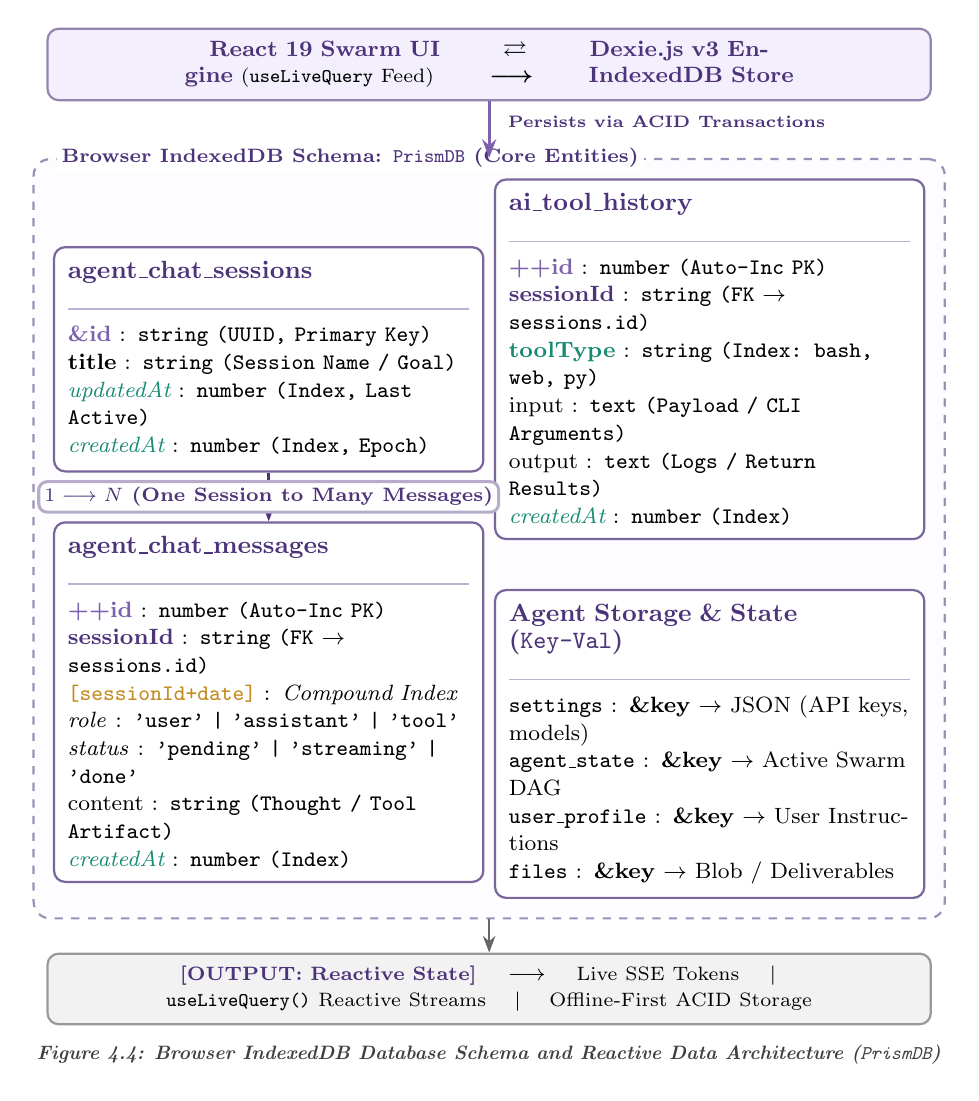
\begin{tikzpicture}[
    font=\sffamily,
    tbl/.style={
        rectangle, draw=lavenderDark!75, line width=0.8pt, fill=white,
        rounded corners=4pt, inner sep=5pt,
        font=\fontsize{8.2}{10.0}\selectfont, align=left
    },
    sysbox/.style={
        rectangle, draw=lavenderDark!65, line width=0.8pt, fill=lavenderLight,
        rounded corners=4pt, inner sep=4.5pt, align=center,
        font=\fontsize{7.8}{9.5}\selectfont
    },
    arr/.style={-{Stealth[scale=0.85]}, line width=0.9pt, draw=lavenderDark}
]

    % Left Table 1: Sessions
    \node [tbl, text width=5.1cm] (tsess) at (-2.8, 0) {
        \textbf{\fontsize{8.8}{10.8}\selectfont\color{lavenderDark}agent\_chat\_sessions}\\[0.15em]
        {\color{lavenderMedium!50}\rule{\linewidth}{0.5pt}}\\[0.2em]
        \textbf{\color{lavenderMedium}\&id} : \texttt{string (UUID, Primary Key)}\\
        \textbf{title} : \texttt{string (Session Name / Goal)}\\
        \textit{\color{prismTeal}updatedAt} : \texttt{number (Index, Last Active)}\\
        \textit{\color{prismTeal}createdAt} : \texttt{number (Index, Epoch)}
    };

    % Right Table 1: Tool Execution History
    \node [tbl, text width=5.1cm] (ttool) at (2.8, 0) {
        \textbf{\fontsize{8.8}{10.8}\selectfont\color{lavenderDark}ai\_tool\_history}\\[0.15em]
        {\color{lavenderMedium!50}\rule{\linewidth}{0.5pt}}\\[0.2em]
        \textbf{\color{lavenderMedium}++id} : \texttt{number (Auto-Inc PK)}\\
        \textbf{\color{lavenderDark}sessionId} : \texttt{string (FK $\to$ sessions.id)}\\
        \textbf{\color{prismTeal}toolType} : \texttt{string (Index: bash, web, py)}\\
        input : \texttt{text (Payload / CLI Arguments)}\\
        output : \texttt{text (Logs / Return Results)}\\
        \textit{\color{prismTeal}createdAt} : \texttt{number (Index)}
    };

    % Left Table 2: Messages (strictly below tsess)
    \node [tbl, text width=5.1cm, below=0.62cm of tsess] (tmsg) {
        \textbf{\fontsize{8.8}{10.8}\selectfont\color{lavenderDark}agent\_chat\_messages}\\[0.15em]
        {\color{lavenderMedium!50}\rule{\linewidth}{0.5pt}}\\[0.2em]
        \textbf{\color{lavenderMedium}++id} : \texttt{number (Auto-Inc PK)}\\
        \textbf{\color{lavenderDark}sessionId} : \texttt{string (FK $\to$ sessions.id)}\\
        \texttt{\color{prismGold!90!black}[sessionId+date]} : \textit{Compound Index}\\
        \textit{role} : \texttt{'user' | 'assistant' | 'tool'}\\
        \textit{status} : \texttt{'pending' | 'streaming' | 'done'}\\
        content : \texttt{string (Thought / Tool Artifact)}\\
        \textit{\color{prismTeal}createdAt} : \texttt{number (Index)}
    };

    % Right Table 2: Storage & Settings (strictly below ttool)
    \node [tbl, text width=5.1cm, below=0.62cm of ttool] (tstore) {
        \textbf{\fontsize{8.8}{10.8}\selectfont\color{lavenderDark}Agent Storage \& State (\texttt{Key-Val})}\\[0.15em]
        {\color{lavenderMedium!50}\rule{\linewidth}{0.5pt}}\\[0.2em]
        \texttt{settings} : \textbf{\&key} $\to$ JSON (API keys, models)\\
        \texttt{agent\_state} : \textbf{\&key} $\to$ Active Swarm DAG\\
        \texttt{user\_profile} : \textbf{\&key} $\to$ User Instructions\\
        \texttt{files} : \textbf{\&key} $\to$ Blob / Deliverables
    };

    % 1 -> N Relational Link
    \draw [arr, line width=1.1pt] (tsess.south) --
        node[draw=lavenderDark!40, fill=white, rounded corners=3pt, inner sep=2pt,
             font=\fontsize{6.6}{8.0}\selectfont\bfseries\color{lavenderDark}]
            {$1 \longrightarrow N \text{ (One Session to Many Messages)}$} (tmsg.north);

    % Schema Container Boundary on background layer
    \begin{scope}[on background layer]
    \node [draw=lavenderDark!55, dashed, rounded corners=6pt, line width=0.8pt, fill=lavenderLight!20,
           fit=(tsess) (tmsg) (ttool) (tstore), inner xsep=7pt, inner ysep=7pt] (schema_box) {};
    \end{scope}
    \node [anchor=west, font=\fontsize{7.4}{8.8}\selectfont\bfseries\color{lavenderDark}, fill=white, inner sep=1.8pt]
        at ($(schema_box.north west)+(0.3, 0)$) {Browser IndexedDB Schema: \texttt{PrismDB} (Core Entities)};

    % Top Flow Banner (strictly above schema_box)
    \node [sysbox, text width=10.9cm, fill=lavenderLight, draw=lavenderDark!60, above=0.72cm of schema_box.north] (top_flow) {
        \textbf{\fontsize{8.5}{10.2}\selectfont\color{lavenderDark}React 19 Swarm UI}
        $\;\;\boldsymbol{\rightleftarrows}\;\;$
        \textbf{\fontsize{8.5}{10.2}\selectfont\color{lavenderDark}Dexie.js v3 Engine}
        {\fontsize{7.2}{8.5}\selectfont(\texttt{useLiveQuery} Feed)}
        $\;\;\boldsymbol{\longrightarrow}\;\;$
        \textbf{\fontsize{8.5}{10.2}\selectfont\color{lavenderDark}IndexedDB Store}
    };
    \draw [arr, line width=1.1pt, draw=lavenderMedium] (top_flow.south) -- 
        node[right, font=\fontsize{6.2}{7.2}\selectfont\bfseries\color{lavenderDark}, xshift=3pt, yshift=3pt]{Persists via ACID Transactions} (schema_box.north);

    % Bottom Output Bar (strictly below schema_box)
    \node [sysbox, text width=10.9cm, fill=black!5, draw=black!40, below=0.42cm of schema_box.south] (out_bar) {
        \textbf{\fontsize{7.5}{9}\selectfont\color{lavenderDark}[OUTPUT: Reactive State]} $\;\longrightarrow\;$
        \fontsize{7.0}{8.5}\selectfont
        Live SSE Tokens $\;\vert\;$ \texttt{useLiveQuery()} Reactive Streams $\;\vert\;$ Offline-First ACID Storage
    };
    \draw [arr, draw=black!60] (schema_box.south) -- (out_bar.north);

    % Caption
    \node [font=\fontsize{7.0}{8.5}\selectfont\bfseries\color{black!75}, below=0.12cm of out_bar] {
        \textit{Figure 4.4: Browser IndexedDB Database Schema and Reactive Data Architecture (\texttt{PrismDB})}
    };

\end{tikzpicture}%
}
\end{column}

%% ─── RIGHT COLUMN: Glossary (28% Width) ────────────────────────────────────
\begin{column}{0.31\textwidth}
\vspace{-0.15cm}
\adjustbox{max width=\linewidth, max height=0.86\textheight}{%
\begin{tcolorbox}[
    enhanced, arc=4pt,
    colframe=lavenderDark!85,
    colback=lavenderLight,
    boxrule=0.8pt,
    left=5pt, right=5pt, top=5pt, bottom=5pt
]
{\fontsize{8.5}{10}\selectfont\bfseries\color{lavenderDark}\faBookOpen\hspace{4pt}Glossary}\\[-0.1em]
{\color{lavenderMedium}\rule{\linewidth}{0.6pt}}\\[0.35em]

\textbf{\fontsize{7.2}{8.5}\selectfont\color{lavenderDark}1. PrismDB}\\
{\fontsize{6.2}{7.4}\selectfont Client-side IndexedDB storing AI swarm sessions, chat \& tool telemetry.}\\[0.4em]

\textbf{\fontsize{7.2}{8.5}\selectfont\color{lavenderDark}2. Dexie.js v3}\\
{\fontsize{6.2}{7.4}\selectfont TypeScript IDB wrapper handling schema migrations \& ACID transactions.}\\[0.4em]

\textbf{\fontsize{7.2}{8.5}\selectfont\color{lavenderDark}3. PK \& FK Keys}\\
{\fontsize{6.2}{7.4}\selectfont \texttt{\&id} (UUID PK), \texttt{++id} (Auto-Inc PK), and $1\to N$ relational links to sessions.}\\[0.4em]

\textbf{\fontsize{7.2}{8.5}\selectfont\color{lavenderDark}4. Compound Idx}\\
{\fontsize{6.2}{7.4}\selectfont B-tree index \texttt{[session+date]} for instant sub-millisecond query slicing.}\\[0.4em]

\textbf{\fontsize{7.2}{8.5}\selectfont\color{lavenderDark}5. \texttt{useLiveQuery()}}\\
{\fontsize{6.2}{7.4}\selectfont Reactive hook auto-rerendering React UI components on local DB changes.}
\end{tcolorbox}%
}
\end{column}

\end{columns}
\end{frame}



% =============================================================================
% SECTION 4: ALGORITHM
% =============================================================================
\section{Multi-Agent Swarm Algorithm}


% Visual Palette matching the clean presentation algorithm format with Lavender
\setbeamercolor{frametitle}{bg=lavenderDark,fg=white}
\setbeamercolor{author in head/foot}{bg=lavenderDark, fg=white}
\setbeamercolor{title in head/foot}{bg=lavenderMedium, fg=white}
\setbeamercolor{date in head/foot}{bg=lavenderDark, fg=white}

% Plain lavender numbered enumeration and accent bullet points
\setbeamertemplate{enumerate item}{\textbf{\color{lavenderDark}\arabic{enumi}.}}
\setbeamertemplate{enumerate subitem}{\textbf{\color{lavenderDark}\arabic{enumii}.}}
\setbeamertemplate{itemize item}{\color{lavenderAccent}\raisebox{0.1ex}{\scriptsize$\bullet$}}
\setbeamertemplate{itemize subitem}{\color{lavenderAccent}\raisebox{0.1ex}{\scriptsize$\bullet$}}

\begin{frame}[t]{Algorithm}
  \vspace{0.15em}
  {\large\bfseries\color{lavenderDark}Step 1: Data collection and Preprocessing}
  \vspace{0.15em}
  \begin{enumerate}\setlength{\itemsep}{1.2pt}\small
    \item Import and unify benchmark records ($\mathcal{D}$), mapping heterogeneous prompt schemas into a structured format.
    \item Clean the dataset (strip malformed Unicode, redundant whitespace, and duplicate prompt-response pairs).
    \item Standardize continuous features (tokens, complexity, latency) using $z$-score normalization: $z = (x - \mu)/\sigma$.
    \item Split the dataset into:
      \begin{itemize}\setlength{\itemsep}{1pt}
        \item 80\% Training set ($\mathcal{D}_{\text{train}}$)
        \item 10\% Validation set ($\mathcal{D}_{\text{val}}$)
        \item 10\% Testing set ($\mathcal{D}_{\text{test}}$)
      \end{itemize}
  \end{enumerate}
  \vspace{0.35em}
  {\large\bfseries\color{lavenderDark}Step 2: Swarm Graph Construction}
  \vspace{0.15em}
  \begin{enumerate}\setlength{\itemsep}{1.2pt}\small
    \item Define node set $V$: specialized agent personas and MCP tools form individual vertices $v_i \in V$.
    \item Evaluate pairwise capability similarity via Pearson correlation: $s_{ij} = \mathrm{Cov}(\mathbf{x}_i, \mathbf{x}_j)/(\sigma_i \sigma_j)$.
    \item Establish adjacency matrix $\mathbf{A}$: set $A_{ij} = 1$ when pairwise similarity meets threshold ($s_{ij} \ge \tau$), and $A_{ij} = 0$ otherwise.
    \item Construct undirected communication edges $E$ permitting message propagation exclusively between complementary pairings.
  \end{enumerate}
\end{frame}

\begin{frame}[t]{Algorithm}
  \vspace{0.15em}
  {\large\bfseries\color{lavenderDark}Step 3: Graph Attention Network (GAT) Initialization}
  \vspace{0.15em}
  \begin{enumerate}\setlength{\itemsep}{1.2pt}\small
    \item Assign each vertex $v_i \in V$ initial embedding vector $\mathbf{h}_i = \mathbf{x}_i \in \mathbb{R}^d$ describing agent operational scope and tool signatures.
    \item Instantiate weight matrix $\mathbf{W} \in \mathbb{R}^{d' \times d}$ and attention vector $\mathbf{a} \in \mathbb{R}^{2d'}$ via Xavier uniform initialization.
    \item Configure network hyperparameters: learning rate $\eta$, multi-head count $K=4$, and dropout probability $p$.
  \end{enumerate}
  \vspace{0.35em}
  {\large\bfseries\color{lavenderDark}Step 4: Attention-Based Message Passing}
  \vspace{0.15em}
  \begin{enumerate}\setlength{\itemsep}{1.2pt}\small
    \item Compute raw attention coefficients with connected neighbors $v_j \in \mathcal{N}(i)$:
      $$e_{ij} = \mathrm{LeakyReLU}\Big(\mathbf{a}^T \big[\mathbf{W} \mathbf{h}_i \,\Vert\, \mathbf{W} \mathbf{h}_j\big]\Big)$$
      \vspace{-0.3em}
    \item Normalize coefficients via Softmax over $\mathcal{N}(i)$: $\alpha_{ij} = \exp(e_{ij}) / \sum_{k \in \mathcal{N}(i)} \exp(e_{ik})$.
    \item Aggregate multi-head neighborhood features across $K=4$ heads: $\mathbf{h}_i' = \Vert_{k=1}^K \sigma\big(\sum_{j \in \mathcal{N}(i)} \alpha_{ij}^k \mathbf{W}^k \mathbf{h}_j\big)$.
    \item Multi-perspective collaborative attention heads capture:
      \begin{itemize}\setlength{\itemsep}{1pt}
        \item Head 1: Intent \& Query Semantics \quad$\vert$\quad Head 2: Model Capability \& Context
        \item Head 3: Swarm Persona \& Tool Affinity \quad$\vert$\quad Head 4: Safety \& Latency Budget
      \end{itemize}
  \end{enumerate}
\end{frame}

\begin{frame}[t]{Algorithm}
  \vspace{0.15em}
  {\large\bfseries\color{lavenderDark}Step 5: Classification and Multi-Task Loss Computation}
  \vspace{0.15em}
  \begin{enumerate}\setlength{\itemsep}{1.2pt}\small
    \item Route updated representations $\mathbf{h}_i'$ through dual specialized prediction heads:
      \begin{itemize}\setlength{\itemsep}{1pt}
        \item Provider Routing Head: $\hat{\mathbf{y}}_{\text{route}} = \mathrm{Softmax}(\mathbf{W}_{\text{route}} \mathbf{h}' + \mathbf{b}_{\text{route}})$
        \item Agent Dispatch Head: $\hat{y}_{\text{agent}, i} = \mathrm{Sigmoid}(\mathbf{W}_{\text{agent}} \mathbf{h}_i' + b_i)$
      \end{itemize}
    \item Compute unified multi-task loss balancing routing accuracy with minimal swarm over-provisioning:
      $$\mathcal{L}_{\text{class}} = \mathcal{L}_{\text{CE}}(\mathbf{y}_{\text{route}}, \hat{\mathbf{y}}_{\text{route}}) + \lambda \sum_{v \in V} \mathcal{L}_{\text{BCE}}(y_v, \hat{y}_v)$$
      \vspace{-0.3em}
    \item Optimize network parameters using AdamW with cosine learning rate decay and gradient clipping.
  \end{enumerate}
  \vspace{0.3em}
  {\large\bfseries\color{lavenderDark}Step 6: Single-Stage Preference Alignment (ORPO)}
  \vspace{0.15em}
  \begin{enumerate}\setlength{\itemsep}{1.2pt}\small
    \item Attach Low-Rank Adapters (LoRA) $\Delta \mathbf{W} = \frac{\alpha}{r} \mathbf{B}\mathbf{A}$ to base model attention projection layers.
    \item Compute Supervised Fine-Tuning (SFT) loss on favored response $y_w$: $\mathcal{L}_{\mathrm{SFT}} = -\frac{1}{|y_w|} \sum_{t=1}^{|y_w|} \log P(y_{w,t} \mid x, y_{w,<t})$.
    \item Formulate Odds Ratio preference penalty: $\mathcal{L}_{\mathrm{OR}} = -\log \sigma \big(\log [\mathrm{odds}(y_w \mid x) / \mathrm{odds}(y_l \mid x)]\big)$ where $\mathrm{odds}(y \mid x) = \frac{P(y \mid x)}{1 - P(y \mid x)}$.
    \item Jointly optimize unified objective: $\mathcal{L}_{\mathrm{ORPO}} = \mathcal{L}_{\mathrm{SFT}} + \beta \cdot \mathcal{L}_{\mathrm{OR}}$ without separate reward models.
  \end{enumerate}
\end{frame}

\begin{frame}[t]{Algorithm}
  \vspace{0.2em}
  {\large\bfseries\color{lavenderDark}Step 7: Real-Time Runtime Inference and Swarm Execution}
  \vspace{0.25em}
  \begin{enumerate}\setlength{\itemsep}{3pt}\small
    \item Ingest natural language prompt $\mathcal{T}_{\text{user}}$ via Next.js client interface and dispatch to FastAPI Hive Bridge.
    \item Synthesize query feature vector: $\mathbf{x}_{\text{query}} = [\text{TF-IDF} \parallel \text{Dense Embeddings} \parallel \text{Context}]$.
    \item Select optimal provider ($\hat{y}_{\text{provider}} = \mathrm{argmax}(\hat{\mathbf{y}}_{\text{route}})$) and dispatch swarm ($\hat{\mathbf{y}}_{\text{agents}} = \mathbb{I}(\hat{\mathbf{y}}_{\text{dispatch}} \ge \tau_{\text{dispatch}})$).
    \item Formulate task DAG and execute topological sort: $\pi = \mathrm{TopologicalSort}(\mathcal{G}_{\text{active}})$.
    \item Execute autonomous ReAct swarm loops querying Model Context Protocol (MCP) tool endpoints (Filesystem, Terminal, Browser, GitHub) until sub-tasks resolve.
    \item Enforce calibrated safety gating: evaluate completion safety log-odds score against policy threshold $\tau_{\text{safety}}$ to intercept prompt injection.
    \item Deliver real-time response: stream verified tokens live via Server-Sent Events (SSE) and commit conversation state locally to \texttt{PrismDB} (Dexie.js).
  \end{enumerate}
\end{frame}

\begin{frame}[t]{Algorithm}
  \vspace{0.2em}
  {\large\bfseries\color{lavenderDark}Step 8: Model Evaluation and Calibration}
  \vspace{0.2em}
  \begin{enumerate}\setlength{\itemsep}{2pt}\small
    \item Benchmark trained routing and alignment models against holdout validation ($\mathcal{D}_{\text{val}}$) and test ($\mathcal{D}_{\text{test}}$) splits.
    \item Compute comprehensive quantitative validation metrics:
      \begin{itemize}\setlength{\itemsep}{1.5pt}
        \item Routing Accuracy \& Macro-F1: Balanced intent and provider classification across rare classes.
        \item Discrimination Capability (ROC-AUC / AUPRC): Safety gate discrimination under class imbalance.
        \item Expected Calibration Error (ECE): $\mathrm{ECE} = \sum_{m=1}^M \frac{|B_m|}{N} \big|\mathrm{acc}(B_m) - \mathrm{conf}(B_m)\big|$
        \item Regression Precision ($R^2$ / MAE): Predictive fidelity for latency ($\hat{\ell}$) and monetary token cost ($\hat{c}$).
      \end{itemize}
  \end{enumerate}
  \vspace{0.35em}
  {\large\bfseries\color{lavenderDark}Step 9: Visualization, HUD Telemetry \& Monitoring}
  \vspace{0.2em}
  \begin{enumerate}\setlength{\itemsep}{2pt}\small
    \item Generate convergence diagnostics: plot training/validation loss trajectories and ROC frontiers.
    \item Inspect attention heatmaps across $K=4$ GAT heads to identify inter-agent collaboration bottlenecks.
    \item Swarm Telemetry HUD: track live provider routing hit-rates, real-time token cost consumption ($\hat{c}$), per-agent latency profiling ($\hat{\ell}$), and safety policy pass-rates.
  \end{enumerate}
\end{frame}

% Restore Madrid Theme Palette
\setbeamercolor{frametitle}{bg=lavenderDark,fg=white}
\setbeamercolor{author in head/foot}{bg=lavenderDark, fg=white}
\setbeamercolor{title in head/foot}{bg=lavenderMedium, fg=white}
\setbeamercolor{date in head/foot}{bg=lavenderDark, fg=white}
\setbeamertemplate{enumerate item}[default]
\setbeamertemplate{itemize item}{\color{lavenderAccent}$\blacktriangleright$}
\setbeamertemplate{itemize subitem}{\color{lavenderMedium}$\bullet$}

% =============================================================================
% CONCLUSION SLIDE
% =============================================================================
\section{Conclusion}



\begin{frame}[plain]
  \begin{tikzpicture}[remember picture,overlay]
    \fill[prismLight] (current page.north west) rectangle (current page.south east);
  \end{tikzpicture}
  \centering
  \vspace{1.5cm}
  {\Huge \textbf{\color{lavenderDark}Thank You!}}\\[1.0em]
  {\Large \textbf{\color{lavenderMedium}Questions \& Discussion}}\\[1.5em]
  {\normalsize \color{prismDark}
    Nobin Sijo \quad$\vert$\quad Pranav P \quad$\vert$\quad Prasanth P \quad$\vert$\quad Sankar Narayan S\\[0.5em]
    \color{prismSlate}Department of Computer Science \& Engineering\\
    College of Engineering, Karunagappally
  }
\end{frame}

\end{document}
